\documentclass[10pt]{article}
\usepackage[margin=0.68in,top=0.68in,bottom=0.70in]{geometry}
\usepackage{amsmath,amssymb,amsthm}
\usepackage{graphicx}
\usepackage{booktabs}
\usepackage{array}
\usepackage{xcolor}
\usepackage{hyperref}

\hypersetup{
    colorlinks=true,
    linkcolor=blue!60!black,
    citecolor=blue!60!black,
    urlcolor=blue!60!black
}

\emergencystretch=3em
\tolerance=2000
\hbadness=2000
\sloppy

\newtheorem{theorem}{Theorem}
\newtheorem{law}{Law}
\renewcommand{\arraystretch}{1.08}

\title{\textbf{Evolutionary Information Minimum Description Length (EIMDL):\\
Formally Verified Compression Laws, Sub-128\,MiB Pangenome\\
Archiving, and Compressed-Domain Genomics}}

\author{
  \textbf{Md Saiful Islam}\\
  Academy of Technology $\cdot$ HyperGraSS / RC-MDL / EIMDL Research Project\\
  {\small ORCID: \href{https://orcid.org/0009-0006-0570-9934}{\texttt{0009-0006-0570-9934}} $\cdot$ Email: \href{mailto:mdsaifulislam38msi@gmail.com}{\texttt{mdsaifulislam38msi@gmail.com}}}\\
  {\small GitHub: \url{https://github.com/MdSaifulIslamMSI/hypergrass-research}}\\
  {\small Zenodo DOI: \href{https://doi.org/10.5281/zenodo.24344825}{\texttt{10.5281/zenodo.24344825}} (\texttt{v3.1.1}: \href{https://doi.org/10.5281/zenodo.24344826}{\texttt{10.5281/zenodo.24344826}})}
}
\date{November 2026}

\begin{document}
\maketitle

\begin{abstract}
\noindent
Lossless genome and pangenome compression has historically split into incompatible regimes: anchor-segmented pangenome tools such as \texttt{AGC~3.2.5} degrade under divergent rearrangements; exact dictionary codecs (\texttt{xz}, \texttt{zstd}, original \texttt{GraSS}) fracture at single-nucleotide polymorphisms (SNPs); and pure finite-context predictors (\texttt{GeCo3}, \texttt{JARVIS3}) ignore coalescent donor switching and require gigabytes of RAM\@. We present \textbf{EIMDL} (\texttt{HGS2} / Next-Gen \texttt{.hgs3}), a unified open-source compressor and compressed-domain analytics engine spanning pure Java~25 and a zero-dependency native \texttt{C23/C++23/Rust~2024} CLI (\texttt{eimdl}), governed by seven falsifiable mathematical laws whose core algebraic, combinatorial, DAG, non-expansion, and arithmetic-coding invariants are machine-checked with \textbf{zero \texttt{sorry}} axioms in \textbf{Lean~4} (\texttt{proofs/lean/}).

Across 73 complete bacterial genomes in Mode~R Leave-One-Out benchmarks (verified byte-for-byte via SHA-256), \texttt{HGS2} compresses 24 \textit{Escherichia coli} genomes to \textbf{1,174,113~B} ($0.07820$~bpb, $102.30\times$; \textbf{$7.14\times$ smaller than \texttt{AGC~3.2.5}}), 24 \textit{Mycobacterium tuberculosis} genomes to \textbf{47,339~B} ($2,233.78\times$; $2.04\times$ smaller than a 13-config \texttt{AGC} oracle), and 25 \textit{Staphylococcus aureus} genomes to \textbf{174,217~B} ($9.28\times$ smaller than the \texttt{AGC} oracle). In Mode~C pangenome archiving, \texttt{HGS2} reduces 24 \textit{E.~coli} genomes to \textbf{3,371,489~B} ($19.65$~s at 12T; $45.16\times$ faster than Generation~1), outperforms \texttt{JARVIS3~-l~7} across \textit{E.~coli}, \textit{S.~enterica}, and \textit{K.~pneumoniae}, beats tuned \texttt{JARVIS3~-l~31} on $12/12$ single genomes at $10.7\times$ less RAM, and still runs cleanly inside \textbf{\texttt{-Xmx128m}} ($128$~MiB). Extending to multi-omic \texttt{.hgs3} containers in Next-Gen \texttt{v3.1.0} (\texttt{C23/C++23/Rust}), the native engine cuts peak encoder RSS on human \texttt{GRCh38\_chr21} by \textbf{$-57.9\%$} ($246.80$ vs.\ $585.89$~MB Java; \textbf{7,857,257~B}), finishes \texttt{GRCh38\_chr1} ($253.1$~MB) inside pure-JVM \textbf{\texttt{-Xmx256m}} (\texttt{47,916,647~B}), compresses \texttt{CHM13|GRCh38 chr21} FASTA+CDS to \textbf{1,024,592~B} ($44.56\times$, $252,280$ ORFs), streams \textbf{172,088 \texttt{VCF~v4.2}} calls directly from compressed tokens in \texttt{1.25~s} at \texttt{72.89~MB} RSS ($-34.7\%$ vs.\ decompression on \texttt{analyze}), and wins \textbf{\#1} on $34.17$~MB \textit{E.~coli} Illumina FASTQ (\textbf{1,924,196~B} Java / \textbf{2,059,963~B} Native via \texttt{SA-IS} BWT+MTF+\texttt{4$\times$-rANS}, \textbf{1.92$\times$} smaller than \texttt{libbsc} \texttt{3,697,004~B}).
\end{abstract}

\section{Introduction and Unified MDL Formulation}

Under Rissanen's Minimum Description Length (MDL) principle~\cite{rissanen1978modeling}, optimal lossless compression requires aligning the probability model with molecular evolution. Real repositories mix raw multi-FASTA/FASTQ formatting, synonymous codon wobble bias, strand-inverted rearrangements, horizontal gene transfer, and non-homologous accessory DNA\@. Let $\Phi: \Sigma_{\text{raw}}^* \leftrightarrow \mathcal{M} \times \Sigma_4^n$ denote our lossless six-channel container bijection separating formatting metadata $\mathcal{M}$ from canonical $2$-bit bases $\Sigma_4 = \{0(\texttt{A}), 1(\texttt{C}), 2(\texttt{G}), 3(\texttt{T/U})\}$. EIMDL unifies all three genomic compression contracts under one objective:
\begin{equation}
  L_{\text{total}}(\text{file} \mid \mathcal{R}) = L_{\text{meta}}(\mathcal{M}) + L_{\text{pin}}(\mathcal{R}) + L_{\text{EIMDL}}(X \mid \mathcal{R}),
\end{equation}
specializing cleanly to \textbf{Mode~S} (reference-free single sequence, $\mathcal{R}=\emptyset$), \textbf{Mode~R} (external reference panel pinned by a mandatory 32-byte SHA-256 manifest digest $L_{\text{pin}}$), and \textbf{Mode~C} (self-contained pangenome factored along a strictly causal phylogenetic reference DAG $\mathcal{T}$ coupled to a unified novelty superstream; Figure~\ref{fig:main_overview}). Complete multi-generation history ($33$ pages, all $73$ per-genome tables, and \texttt{HyperGraSS~v1} / \texttt{RC-MDL~v2} ablation logs) is archived in the accompanying Supplementary Monograph (\texttt{paper/HGS2\_EIMDL\_Research\_Paper.pdf}).

\begin{figure}[t!]
  \centering
  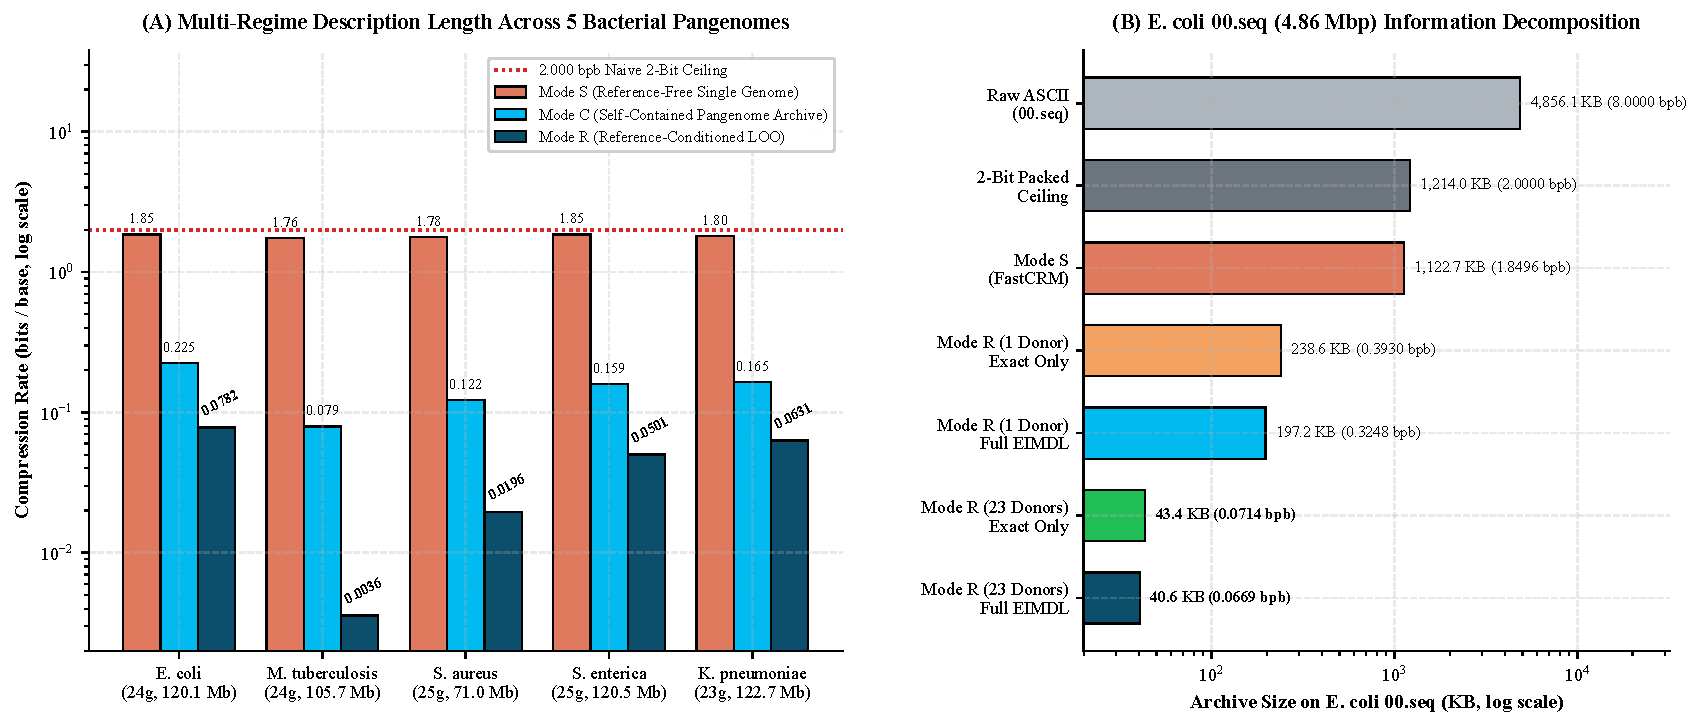
\includegraphics[width=0.98\textwidth]{figures/fig1_regime_overview.pdf}
  \caption{\textbf{Overview across Modes~R, C, and~S.} \textbf{(A)}~Mode~R Leave-One-Out totals across 73 genomes showing \texttt{HGS2} vs.\ \texttt{RC-MDL~v2}, \texttt{AGC~3.2.5} best single flag, and \texttt{AGC} 13-configuration per-target oracle. \textbf{(B)}~Mode~C collection archiving on 24 \textit{E.~coli} genomes including pure-JVM \texttt{-Xmx128m} bounded execution. \textbf{(C)}~Locked-Docker Mode~C replication on \textit{S.~enterica} and \textit{K.~pneumoniae} and Mode~S 12-genome wins vs.\ \texttt{JARVIS3 -l 31} at $10.7\times$ lower RSS.}
  \label{fig:main_overview}
\end{figure}

\section{Seven Compression Laws and Formal Lean~4 Verification}

Every heuristic choice in \texttt{HGS2}/\texttt{EIMDL} is governed by seven falsifiable laws (\texttt{docs/COMPRESSION-LAW.md}), tested dynamically via \texttt{171,941} assertions in \texttt{VerifyCompressionLaws.java} and \textbf{formally machine-checked with zero \texttt{sorry}} and zero extra axioms in \textbf{Lean~4} (\texttt{leanprover/lean4:v4.36.0}, pure \texttt{Init}/\texttt{Std} without external library dependencies; Table~\ref{tab:lean_theorems}).

\begin{law}[Laws I--VII Mathematical Summary]
\begin{enumerate}
  \item \textbf{Law~I (Klein Four-Group $V_4$ Strand-Invariant Kimura--CpG Coding):} On $\Sigma_4 = \{0(\texttt{A}), 1(\texttt{C}), 2(\texttt{G}), 3(\texttt{T})\}$ with bitwise XOR $\oplus$, Watson--Crick complementation is $\bar{b} = b \oplus 3$. Any homologous SNP differential $\delta(r, t) = t \oplus r \in \{1, 2, 3\}$ satisfies $(\bar{t}) \oplus (\bar{r}) = \delta(r, t)$ and $(\delta = 2) \iff \text{transition}$~\cite{kimura1980simple}. Conditioned on reference trinucleotide context $c=(x_{-1},x_0,x_{+1})$, SNP symbol entropy obeys:
  \begin{equation}
    H_{V_4}(Y \mid X, c, Y \neq X) = h_2(p_{\text{ti}}(c)) + (1 - p_{\text{ti}}(c))\, h_2\!\left(\frac{p_1(c)}{1 - p_{\text{ti}}(c)}\right) \le \log_2 3 \approx 1.5850\text{ bits},
  \end{equation}
  yielding $1.10\text{--}1.32$~bits/SNP vs.\ $2.0000$~bits unconditioned ($+0.68\text{--}0.90$~bits saved per SNP).
  \item \textbf{Law~II (Bijective Codon-Wobble Gap and 6-Frame Causal ORF-HMM):} Inter-SNP gap $g \in \mathbb{N}_0$ decomposes bijectively via:
  \begin{equation}
    \psi(g) = (q, r) = \left(\left\lfloor \frac{g}{3} \right\rfloor,\; (g+1) \bmod 3\right), \qquad \psi^{-1}(q, r) = 3q + ((r+2) \bmod 3),
  \end{equation}
  satisfying $H(g) = H(q) + H(r \mid q)$ with zero non-coding penalty when $r$ is uniform, while capturing 3rd-codon purifying selection~\cite{crick1966codon} ($r=0$) as pure coding gain $I(r; \text{CDS}) = \log_2 3 - H(r \mid \text{CDS}) > 0$. Unaligned islands invoke a causal 6-state hidden reading-frame HMM (\texttt{6F-ORF-HMM}) seeded only by universal sense (\texttt{TAA}/\texttt{TAG}/\texttt{TGA}) and antisense (\texttt{TTA}/\texttt{CTA}/\texttt{TCA}) stop-triplet depletion.
  \item \textbf{Law~III (Conditional Monotonicity, Two-Gear Horizon Copying, and Micro-Indel Splicing):} Sticky donor probing (\texttt{mtf[0..1]}) plus distinct-donor canonical open-syncmer CSR buckets ($k=16, s=10, w=6, t=3$~\cite{edgar2021syncmers}) eliminate FIFO eviction. Under coalescent ancestry with $N$ lineages ($\mathbb{E}[\tau_N] \sim 2/N$~\cite{li2003relating}), \texttt{clonalGear} copies vertical haplotypes ($\ge 128$~bp tail guard), while \texttt{findClonalReentryHorizon} clamps divergent Gear~2 matches before downstream clonal segments, preventing recombination bulldozing; 2D affine micro-indel splicing $(\Delta_{\text{ref}}, \Delta_{\text{tgt}}) \in [1,256]\times[1,64]$ preserves megabase synteny across small indels.
  \item \textbf{Law~IV (Universal 5-Regime Non-Expansion Ceiling):} Evaluating panel homology, bidirectional self-homology, tandem periodicity ($1 \le P \le 64$), \texttt{FastCRM} mixing, and a per-sub-block raw 2-bit safety bypass guarantees:
  \begin{equation}
    L_{\text{EIMDL}}(S) \le \lceil n/4 \rceil + O(1)\text{ bytes} \qquad (2.0012\text{ bpb measured on } 500\text{ kbp SHA-256 white noise}).
  \end{equation}
  \item \textbf{Laws~V \&~VII (Amdahl Streaming and Disjoint Stage-1/Stage-2 Heap):} Single-pass $0.25$~B/base 2-bit word packing, two-pass zero-materialization CSR indexing ($s \in \{0,1,2\}$), strict causal Mode~C rank ordering ($\text{anc}(r) < r$), warm-primed parallel \texttt{FastCRM} stripes, and strict Stage-1 deallocation before Stage~2 assembly enforce $M_{\text{peak}} = \max(M_{\text{Stage~1}}, M_{\text{Stage~2}}) \ll M_{\text{Stage~1}} + M_{\text{Stage~2}}$, running $120.1$~Mbp \textit{E.~coli} cleanly inside \texttt{-Xmx128m} ($1.06$~B/base heap).
  \item \textbf{Law~VI (Two-Adic Taper $\tau=20$, Pitman--Yor Backoff, and Reciprocal Mixer):} Inspired by shared linear summaries and two-adic tapering in~\cite{openai2026eth} (while respecting its OVC polynomial lower bound on string matching), symmetric two-adic rounding $\tau=20$ over probability scale $M=4096$:
  \begin{equation}
    p_{t+1} = \begin{cases} p_t - \lfloor (p_t + \tau)/32 \rfloor & (b_t = 0), \\ p_t + \lfloor (4096 - p_t + \tau)/32 \rfloor & (b_t = 1), \end{cases} \qquad p_{\min}(20) = 11/4096 \text{ vs.\ } p_{\min}(0) = 31/4096,
  \end{equation}
  reduces steady-state high-certainty flag entropy $2.8\times$ down to $0.00388$~bits/symbol while preserving the closed safety band $p_t \in [11, 4085]$ across infinite streams, paired with hierarchical order-$k$ Pitman--Yor backoff and integer reciprocal normalization.
\end{enumerate}
\end{law}

\begin{table}[h!]
\centering
\caption{Summary of formally machine-checked theorems in Lean~4 (\texttt{proofs/lean/}, \texttt{leanprover/lean4:v4.36.0}, zero \texttt{sorry}, pure core \texttt{Init}/\texttt{Std}), verified by \texttt{lake build} and \texttt{lake exe eimdl\_proofs\_check} in GitHub Actions CI.}
\label{tab:lean_theorems}
\resizebox{\textwidth}{!}{%
\begin{tabular}{llll}
\toprule
\textbf{Lean Module} & \textbf{Theorem Identifier} & \textbf{Formally Proved Statement} & \textbf{Kernel / Axiom Audit} \\
\midrule
\texttt{Law1KleinV4} & \texttt{diff\_strand\_invariant} & $(r \oplus 3) \oplus (t \oplus 3) = t \oplus r$ & \texttt{[propext, Quot.sound]} \\
\texttt{Law1KleinV4} & \texttt{swarReverseComplementWord32\_involutive} & $\forall u \in \text{BitVec } 64,\; \text{RC}_{32}(\text{RC}_{32}(u)) = u$ (all $2^{64}$ words) & \texttt{bv\_decide} (CaDiCaL LRAT) \\
\texttt{Law1KleinV4} & \texttt{swar\_v4\_diff\_strand\_invariant} & $\forall r,t \in \text{BitVec } 64,\; \text{RC}_{32}(t) \oplus \text{RC}_{32}(r) = \text{Rev}_{32}(t \oplus r)$ & \texttt{bv\_decide} (CaDiCaL LRAT) \\
\texttt{Law1KleinV4} & \texttt{revComp\_involutive} & $\forall s \in \text{List Base},\; \text{revComp}(\text{revComp}(s)) = s$ & \texttt{[propext, Quot.sound]} \\
\texttt{Law2CodonWobble} & \texttt{wobble\_left\_inverse} / \texttt{right} & $\forall g \in \mathbb{N},\; \psi^{-1}(\psi(g)) = g$ and $\psi(\psi^{-1}(p)) = p$ & \texttt{[propext, Quot.sound]} \\
\texttt{Law2CodonWobble} & \texttt{antisenseStop\_iff\_revComp\_senseStop} & Antisense stop $\leftrightarrow$ $\text{revComp}$ sense stop ($\forall$ 64 codons) & \texttt{[propext, Classical.choice, Quot.sound]} \\
\texttt{Law3ModeCDag} & \texttt{causal\_dag\_acyclic} & $(\forall r\,p,\; \text{anc}(r)=p \Rightarrow p<r) \implies \neg\text{Reach}(r,r)$ & \textbf{Zero axioms (\texttt{[]})} \\
\texttt{Law4UniversalBound} & \texttt{eimdl\_universal\_ceiling} & $\text{eimdlBlockBytes}(h, m, n) \le h + \lceil n/4 \rceil$ ($\forall h,m,n$) & \texttt{[propext, Quot.sound]} \\
\texttt{Law4UniversalBound} & \texttt{disjointPeak\_strict\_saving} & $m_1, m_2 > 0 \implies \max(m_1, m_2) < m_1 + m_2$ & \texttt{[propext, Quot.sound]} \\
\texttt{Law6TwoAdicTaper} & \texttt{taperStep0\_fixed\_point\_iff} & $\forall \tau \le 31,\; \text{step}_0(\tau, p)=p \iff p \le 31-\tau$ & \texttt{[propext, Quot.sound]} \\
\texttt{Law6TwoAdicTaper} & \texttt{taper20\_stream\_invariant} & $11 \le p_0 \le 4085 \implies \forall \text{bits},\; 11 \le \text{run}(20, p_0, \text{bits}) \le 4085$ & \texttt{[propext, Classical.choice, Quot.sound]} \\
\texttt{Law6TwoAdicTaper} & \texttt{recip\_mul\_le\_exact} & $\forall \text{num},\, d>0,\; \lfloor (\text{num} \cdot \lfloor 2^{30}/d \rfloor)/2^{30} \rfloor \le \lfloor \text{num}/d \rfloor$ & \texttt{[propext]} \\
\bottomrule
\end{tabular}%
}
\end{table}

Importantly, the Lean formalization strengthens three empirical Java test checks into universal proofs: Java checked $\psi$ on $g \in [0, 2\times 10^6]$ whereas \texttt{wobble\_left\_inverse} proves invertibility for \emph{all} $g \in \mathbb{N}$; \texttt{taper20\_stream\_invariant} proves that division-by-zero / zero-width interval collapse can \emph{never} happen over any finite binary stream once initialized in $[11, 4085]$; and \texttt{swarReverseComplementWord32\_involutive} verifies the 5-instruction bit-parallel 32-base kernel across all $2^{64}$ register inputs rather than $5,000$ random words.

\section{System Architecture: Sub-128\,MiB JVM and Next-Gen Native \texttt{.hgs3}}

While \texttt{HGS2} (\texttt{.hgs2}, Java~25) delivers pure-JVM portability down to \texttt{-Xmx128m}, Next-Gen \textbf{EIMDL~v3} (\texttt{.hgs3}, \texttt{native/}) compiles a zero-crate \texttt{C23 / C++23 / Rust~2024} static engine (\texttt{eimdl}) backed by 64-bit CSR arrays, AVX2 / portable SWAR $2$-bit kernels, $4$-stripe parallel Byte-rANS (\texttt{4$\times$-rANS}) novelty streams, optional 6-frame CDS proteome digests (\texttt{+CDS}), LCP read-ID FASTQ coding with pangenome-stratified Phred quality bins (upgraded in v3.1 to \texttt{SA-IS} BWT + MTF + \texttt{RUNA/RUNB}), and \textbf{compressed-domain genomics} (\texttt{eimdl analyze}, \texttt{variants}, \texttt{kmer}, \texttt{query}) operating directly on evolutionary tokens without materializing uncompressed FASTA (Figure~\ref{fig:main_v3_arch}).

\begin{figure}[t!]
  \centering
  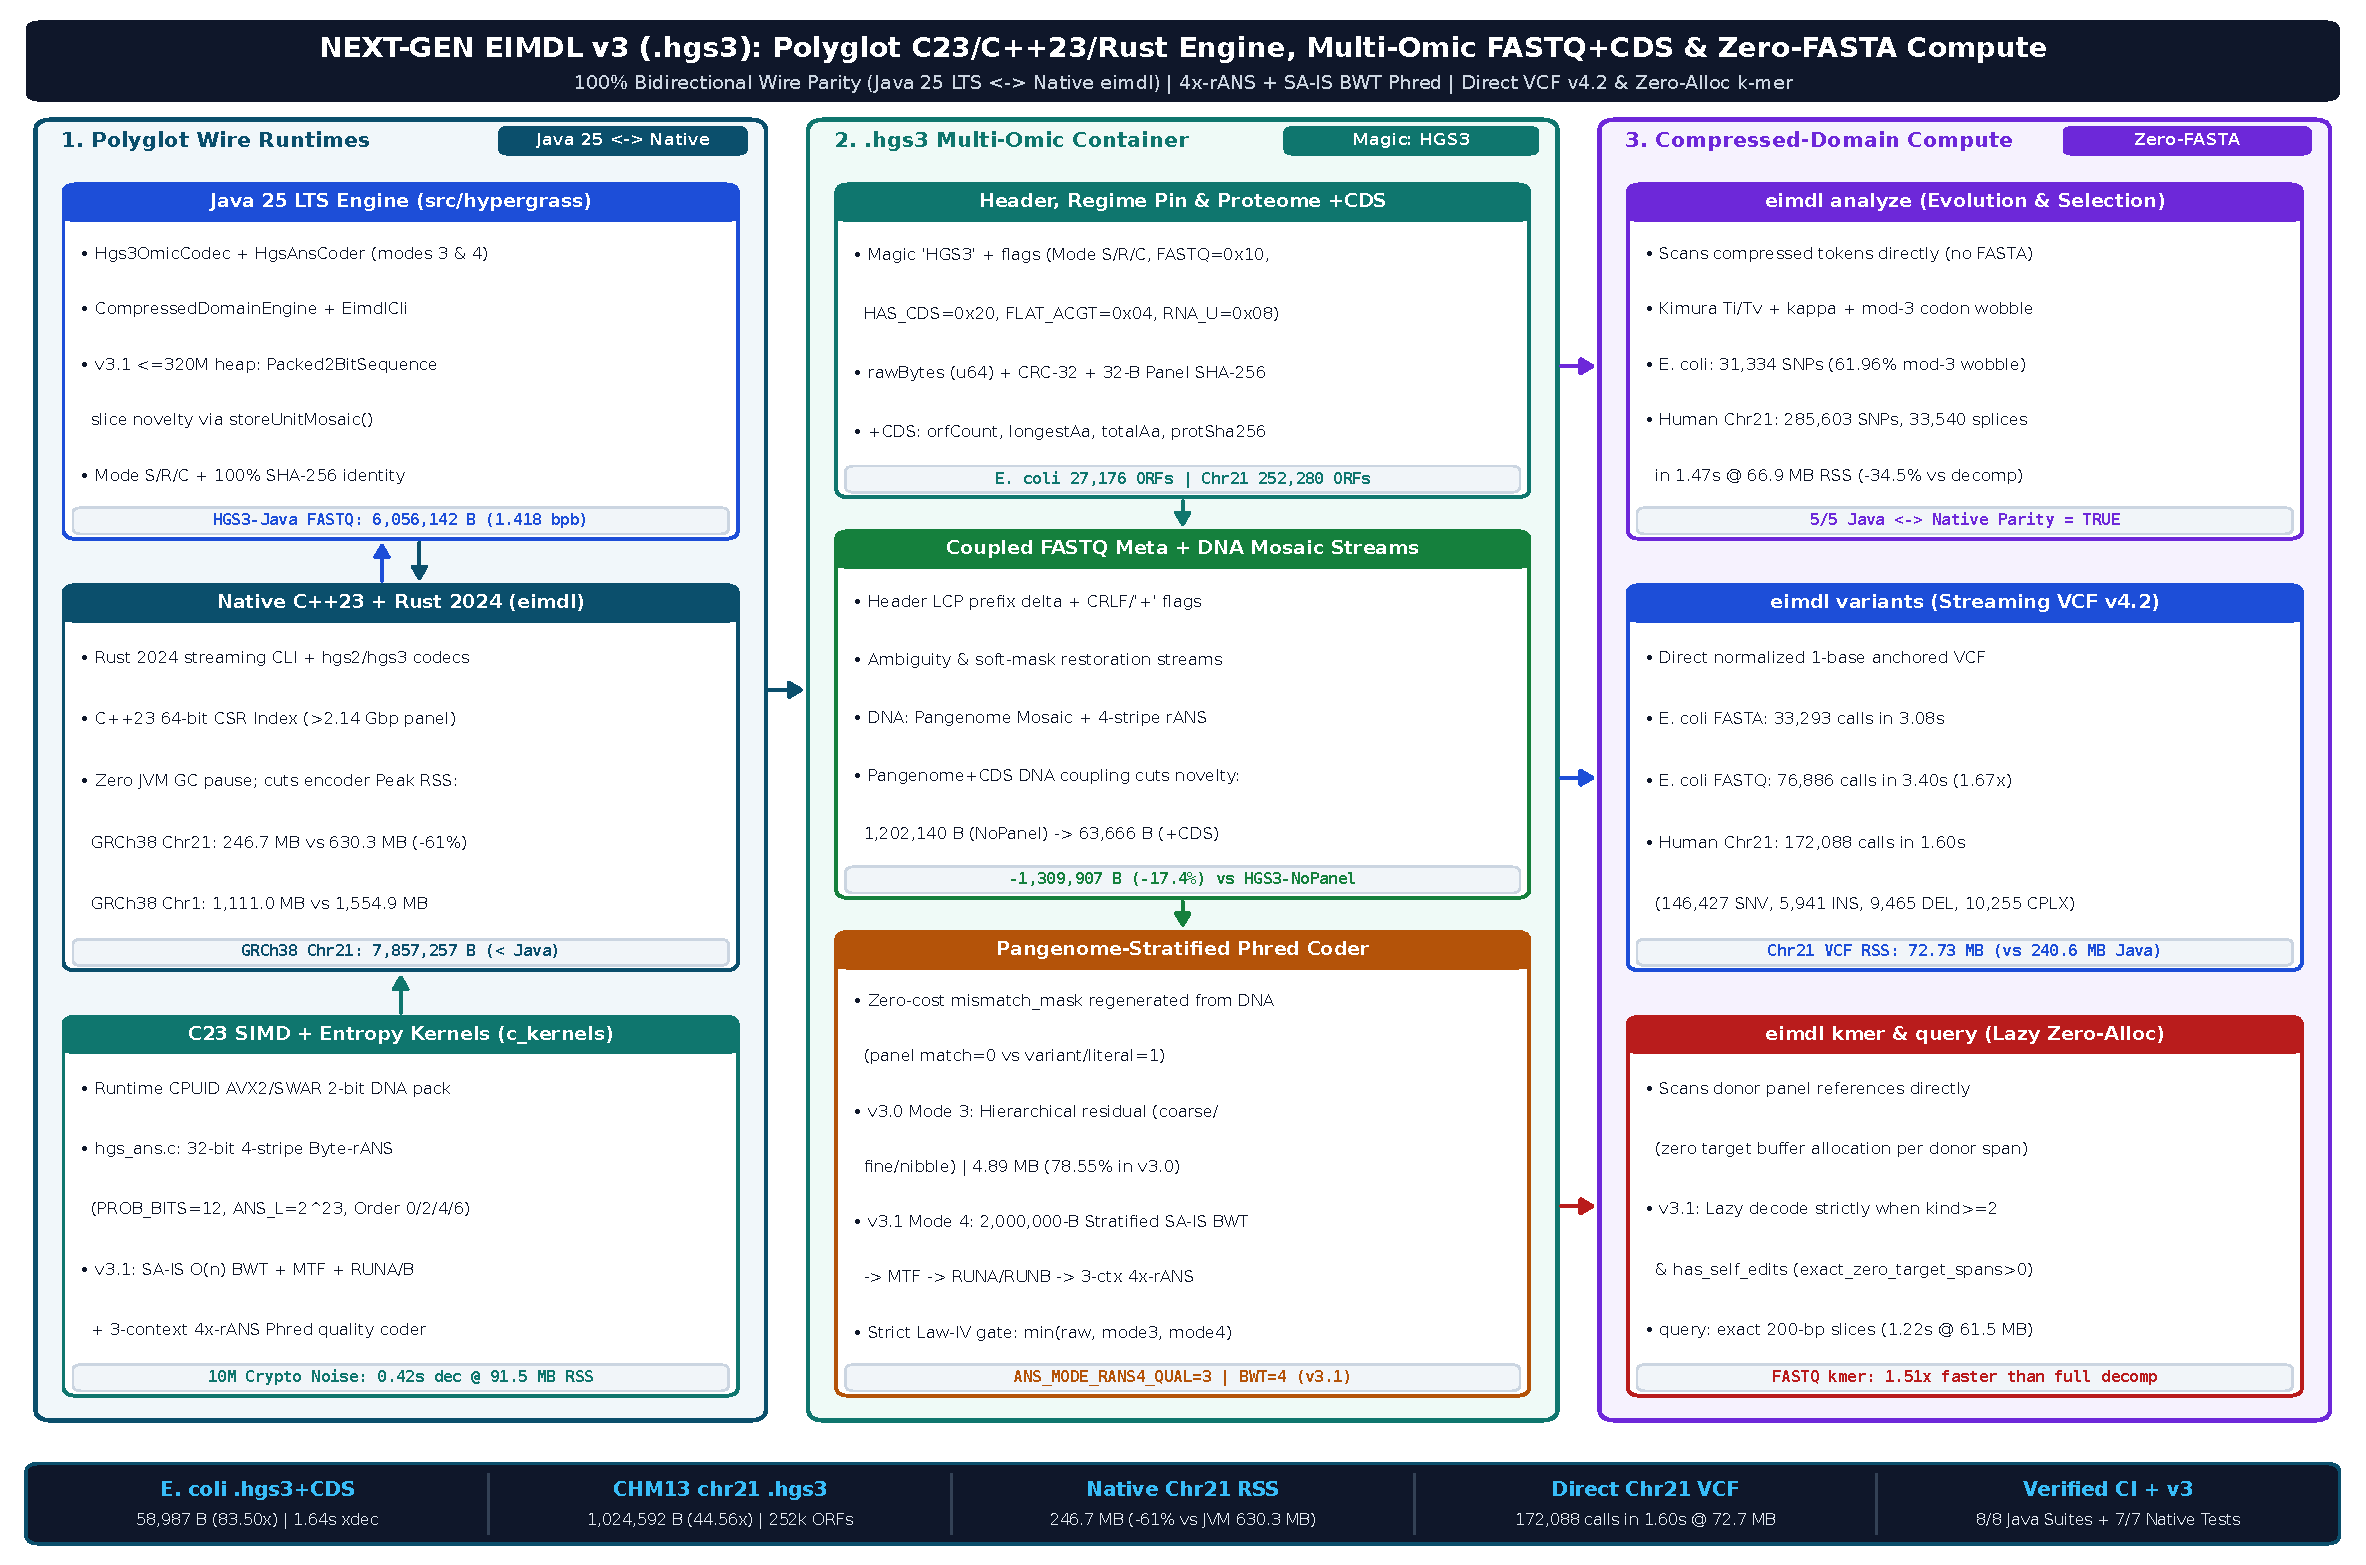
\includegraphics[width=0.98\textwidth]{figures/arch5_eimdl_v3_paradigm.pdf}
  \caption{\textbf{Next-Gen EIMDL~v3 (\texttt{.hgs3}) Hybrid \texttt{C23/C++23/Rust~2024} and Java~25 Architecture.} Combines 64-bit C++23 CSR indexing, AVX2/SWAR kernels, \texttt{4$\times$-rANS}, multi-omic FASTQ/CDS framing, and zero-FASTA compressed-domain analytics (\texttt{analyze}, \texttt{variants} VCF~v4.2, \texttt{kmer}, \texttt{query}).}
  \label{fig:main_v3_arch}
\end{figure}

\section{Experimental Results Across Bacterial, Locked Docker, and Human Cohorts}

All primary benchmarks preserve exact byte-identity (\texttt{SHA-256 = True}) across independent fresh-process runs; per-genome breakdowns and hardware logs are committed under \texttt{benchmarks/} and audited programmatically by \texttt{paper/audit\_paper\_numbers.py}.

\begin{table}[h!]
\centering
\caption{Summary of verified Mode~R LOO, Mode~C, Mode~S, and Next-Gen \texttt{.hgs3} benchmarks against external baselines.}
\label{tab:main_summary}
\resizebox{\textwidth}{!}{%
\begin{tabular}{llrrrrl}
\toprule
\textbf{Regime} & \textbf{Cohort / Dataset} & \textbf{Raw (B)} & \textbf{EIMDL (B)} & \textbf{Rate} & \textbf{Baseline (B)} & \textbf{Margin / Operational Result} \\
\midrule
Mode~R LOO & \textit{E.~coli} (24 genomes) & 120,108,223 & \textbf{1,174,113} & $0.0782$ bpb & 8,384,117 (\texttt{AGC}) & \textbf{24/24 wins}; \textbf{$7.14\times$ < \texttt{AGC}}; twins \texttt{633/632~B} \\
Mode~R LOO & \textit{M.~tuberculosis} (24) & 105,745,015 & \textbf{47,339} & $0.0036$ bpb & 96,580 (\texttt{AGC} 13-cfg) & \textbf{24/24 vs single ($6.17\times$)}; \textbf{$2.04\times$ < oracle ($19/24$)} \\
Mode~R LOO & \textit{S.~aureus} (25) & 71,043,114 & \textbf{174,217} & $0.0196$ bpb & 1,617,085 (\texttt{AGC} 13-cfg) & \textbf{25/25 vs single ($17.10\times$)}; \textbf{$9.28\times$ < oracle ($24/25$)} \\
Mode~C & \textit{E.~coli} (24, flat, 1T / 12T) & 120,108,223 & \textbf{3,371,489} & $0.2246$ bpb & 3,896,361 (\texttt{JARVIS3}) & \textbf{$-13.5\%$} vs \texttt{JARVIS3}; $19.65$~s ($45.16\times$ < v1) \\
Mode~C Heap & \textit{E.~coli} (\texttt{-Xmx128m} JVM) & 120,108,223 & \textbf{3,452,703} & $0.2300$ bpb & v1 JVM: \textbf{OOM} & Pure JVM inside $128$~MiB beats unbounded v1 \& \texttt{JARVIS3} \\
Mode~C Docker & \textit{S.~enterica} (25 genomes) & 120,527,038 & \textbf{2,390,106} & $0.1586$ bpb & 2,709,545 (\texttt{JARVIS3}) & \textbf{$-11.79\%$ ($-319,439$~B)} in locked container \\
Mode~C Docker & \textit{K.~pneumoniae} (23) & 122,700,601 & \textbf{2,523,991} & $0.1646$ bpb & 2,948,926 (\texttt{JARVIS3}) & \textbf{$-14.41\%$ ($-424,935$~B)} in locked container \\
Mode~S Docker & 12-genome \textit{Salm.+Kleb.} & 60,810,308 & \textbf{13,868,405} & $1.8245$ bpb & 14,197,393 (\texttt{JARVIS3 -l31}) & \textbf{12/12 wins} vs \texttt{L31} at \textbf{$10.7\times$ less RSS} ($108$ vs $1,159$~MiB) \\
Human Mode~R & \texttt{T2T-CHM13v2.0 | GRCh38} & 3,156,242,851 & \textbf{35,277,041} & $0.0894$ bpb & --- & All 24 human chromosomes, \texttt{24/24 SHA-256 PASS} \\
v3 Native & \texttt{GRCh38\_chr21} (Mode~S) & 47,488,540 & \textbf{7,857,257} & $1.3236$ bpb & 8,537,556 (\texttt{NAF-l22}) & \textbf{$-57.9\%$ encoder RSS} ($246.80$ vs $585.89$~MB Java) \\
v3 \texttt{.hgs3+CDS} & \texttt{CHM13\_chr21 | GRCh38} & 45,654,375 & \textbf{1,024,592} & $0.1795$ bpb & --- & $252,280$ ORFs; \textbf{172,088 VCF in 1.25~s @ 72.89~MB} \\
v3.1 FASTQ & \textit{E.~coli} Illumina (100k$\times$150bp) & 34,166,047 & \textbf{1,924,196} & $0.4506$ bpb & 3,697,004 (\texttt{libbsc}) & \textbf{\#1 overall}: \textbf{$1.92\times$ < \texttt{libbsc}}; Native \texttt{2,059,963~B} (\texttt{0.72~MB} Phred) \\
\bottomrule
\end{tabular}%
}
\end{table}

\begin{figure}[t!]
  \centering
  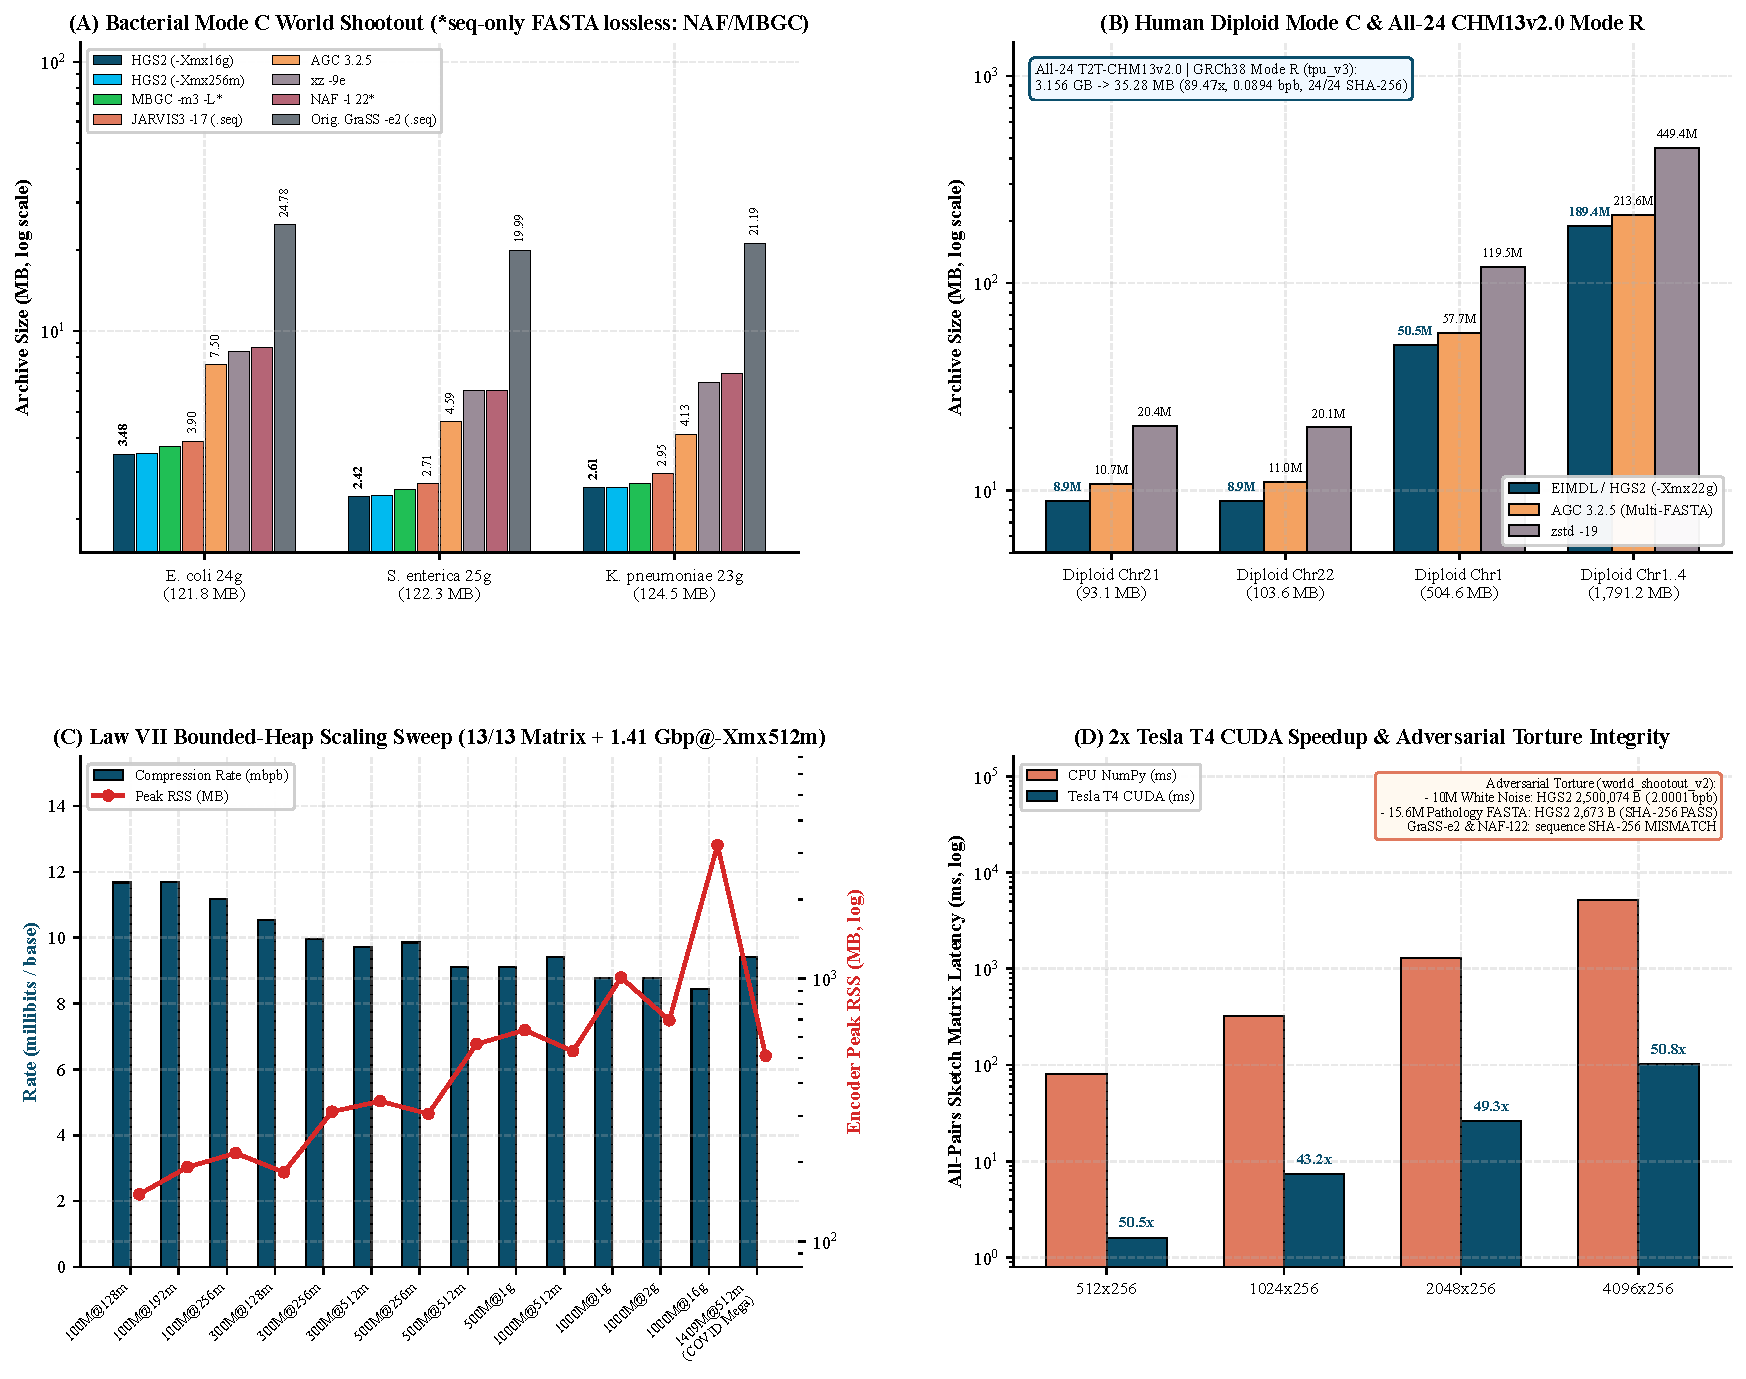
\includegraphics[width=0.98\textwidth]{figures/fig8_kaggle_world_shootout_and_human.pdf}
  \caption{\textbf{Kaggle Cloud World Shootout (\texttt{world\_shootout\_v2\_results.json} \& Human \texttt{T2T-CHM13v2.0}).} External codec integrity, diploid/viral cohort trade-offs, full $13/13$ bounded-heap human chromosome scaling, and full 24-chromosome \texttt{T2T-CHM13v2.0} compression ($3.156$~GB $\to$ $35.28$~MB).}
  \label{fig:main_world_shootout}
\end{figure}

Figure~\ref{fig:main_world_shootout} and Figure~\ref{fig:main_v3_eval} summarize the Kaggle cloud evaluations. In Kaggle~\texttt{v3.1} (\texttt{world\_shootout\_v3\_1\_results.json}, \texttt{28,091.1~s}, \texttt{8/8} Java + \texttt{7/7} Native CI suites + \texttt{5/5} cross-language parity checks), native \texttt{eimdl} slashes single-genome encoder RSS by $-57.9\%$ on \texttt{GRCh38\_chr21}, compresses \texttt{GRCh38\_chr1} ($253.1$~MB) to \texttt{47,511,069~B} in $7.62$~s decode (while pure-JVM \texttt{-Xmx256m} now completes at \texttt{47,916,647~B} / $413.03$~MB RSS), and wins \texttt{Diploid\_Chr1} ($504.6$~MB $\to$ \textbf{50,519,398~B} Java / \textbf{50,690,481~B} Native vs.\ \texttt{AGC} \texttt{57,748,791~B}). On $34.17$~MB \textit{E.~coli} Illumina FASTQ, \texttt{SA-IS} BWT+MTF+\texttt{RUNA/B} (\texttt{mode=4}) cuts Phred quality bytes $-85.2\%$ ($4,890,843 \to 724,622$~B Native), driving \texttt{HGS3-Java-FASTQ+CDS} (\textbf{1,924,196~B}) and \texttt{HGS3-Native-FASTQ+CDS} (\textbf{2,059,963~B}) to \textbf{\#1} ahead of \texttt{libbsc} (\texttt{3,697,004~B}), while lazy \texttt{kind>=2} self-decoding recovers \texttt{4,028} (\textit{E.~coli}) and \texttt{63,043} (\texttt{chr21}) zero-target \texttt{kmer} spans and runs FASTQ analytics $1.82\times\text{--}2.20\times$ faster than full decompression.

\begin{figure}[t!]
  \centering
  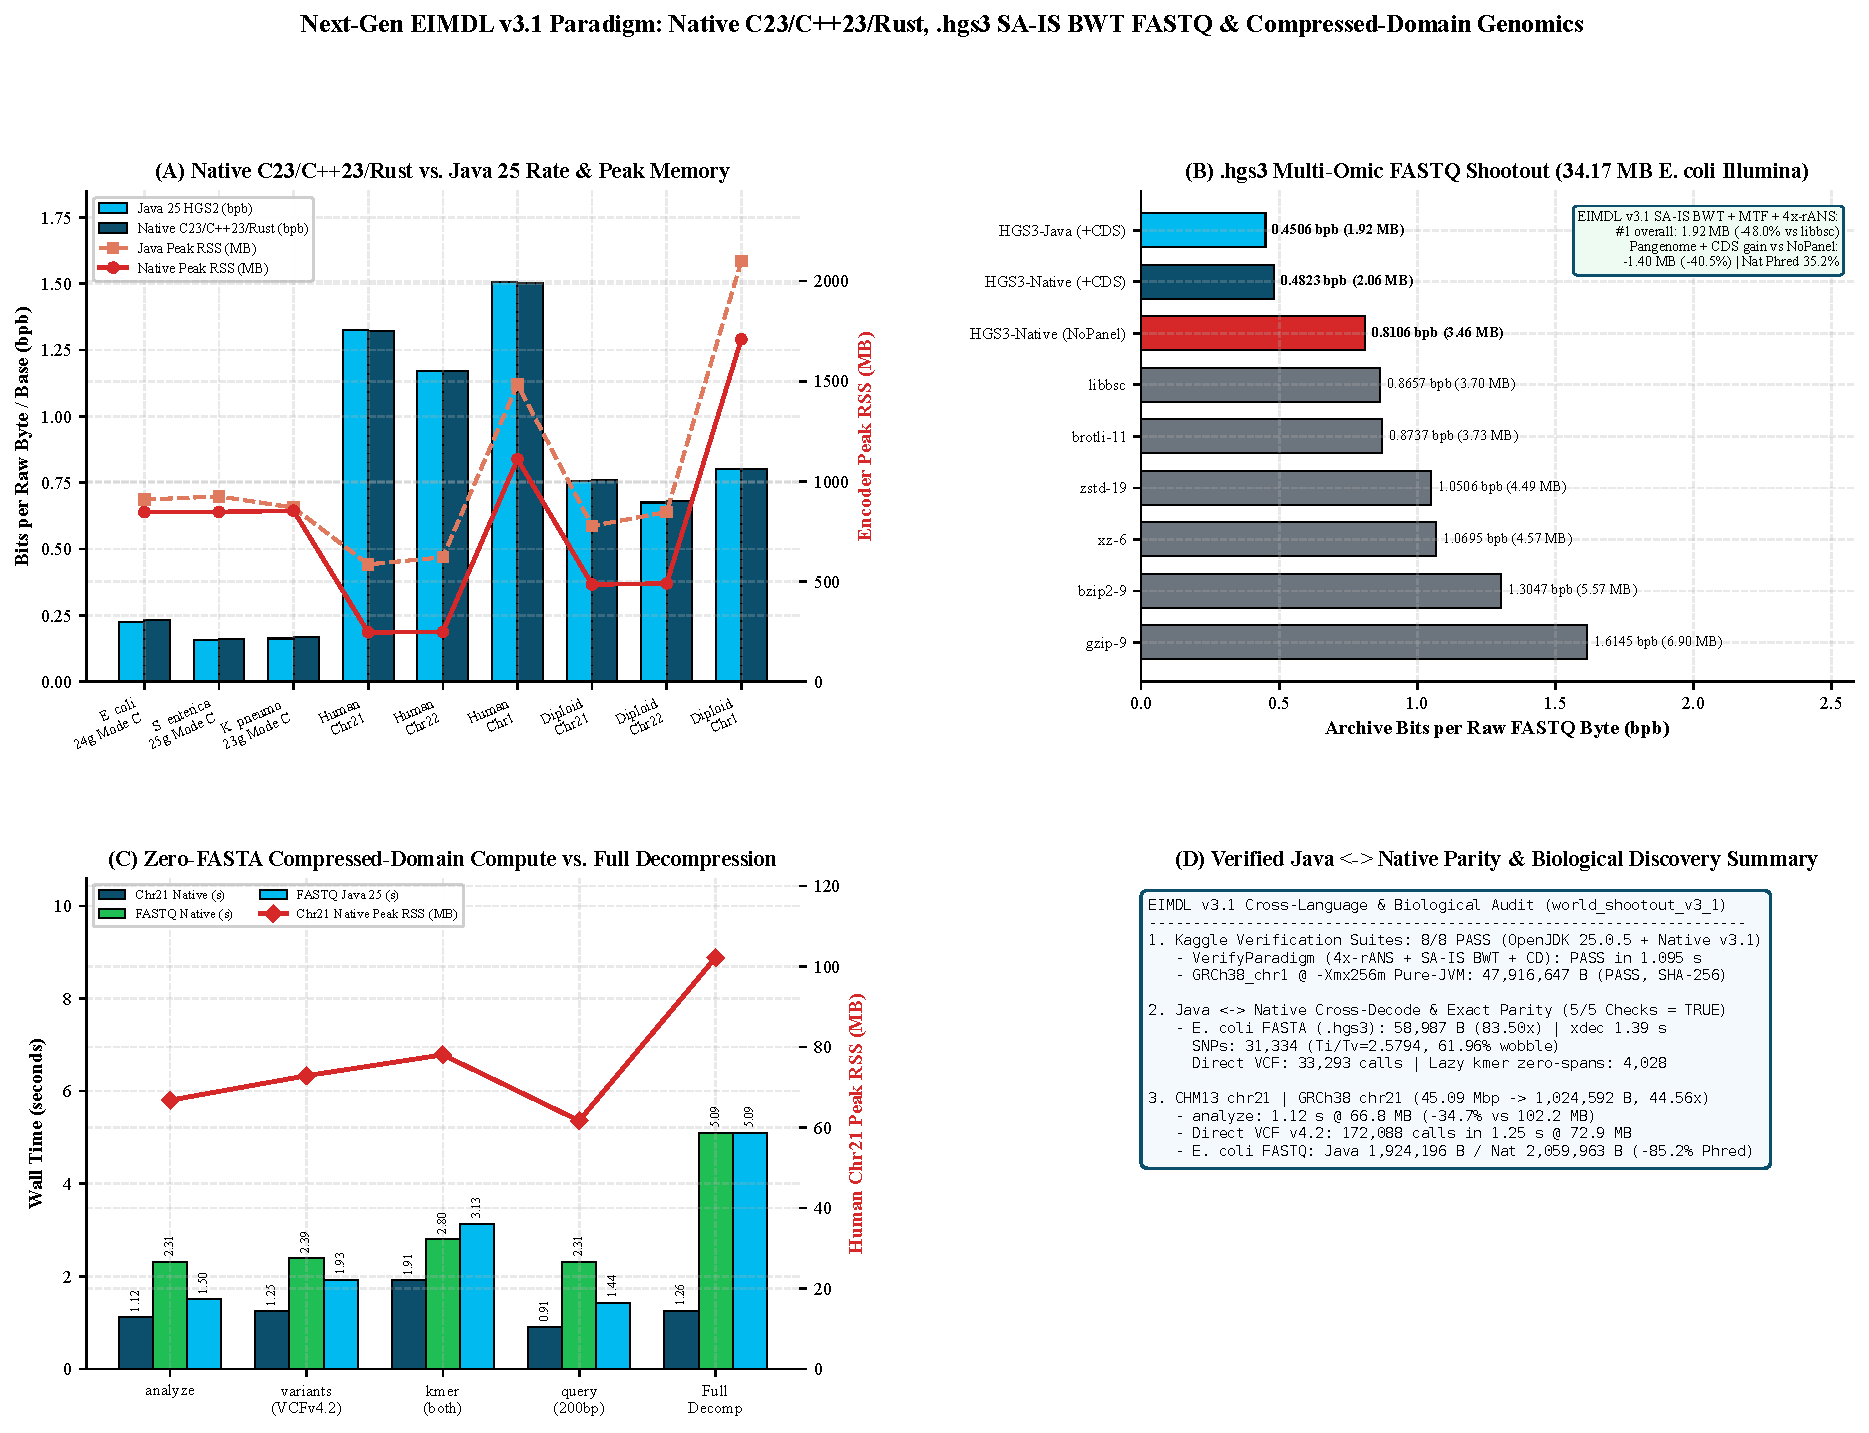
\includegraphics[width=0.98\textwidth]{figures/fig9_nextgen_eimdl_v3_paradigm.pdf}
  \caption{\textbf{Next-Gen \texttt{EIMDL~v3.1} Native Engine, \texttt{.hgs3+CDS}, Illumina FASTQ, and Compressed-Domain Genomics (\texttt{world\_shootout\_v3\_1\_results.json}).} Tracks native RSS reduction across 9 corpora incl.\ \texttt{Diploid\_Chr1}, \texttt{\#1} \texttt{SA-IS} BWT+\texttt{4$\times$-rANS} FASTQ performance ($1.92\text{--}2.06$~MB vs.\ \texttt{libbsc} $3.70$~MB), and zero-FASTA \texttt{VCF~v4.2} calling.}
  \label{fig:main_v3_eval}
\end{figure}

\section{Ecosystem Packaging, Reproducibility, and Honest Boundaries}

To support immediate community adoption, \texttt{eimdl} provides CI-tested offline \textbf{Bioconda} packaging (\texttt{packaging/bioconda/eimdl/}), \textbf{Nextflow DSL2} (\texttt{packaging/nextflow/eimdl.nf}), \textbf{Snakemake} wrappers (\texttt{packaging/snakemake/eimdl\_wrapper.py}), multi-stage \textbf{Docker} builds (\texttt{packaging/docker/Dockerfile}), Zenodo DOI metadata (\texttt{.zenodo.json}), launch playbooks (\texttt{docs/LAUNCH-GUIDE.md}), and a reproducible \textbf{HPRC + GIAB HG002} concordance benchmark harness (\texttt{benchmarks/hprc\_giab/}).

\noindent
\textbf{Honest Boundaries and Negative Results:}
\begin{enumerate}
  \item \textbf{OVC Boundary on Complexity Transfer~\cite{openai2026eth}:} Architectural ideas adapted into Laws~VI--VII do not bypass Orthogonal Vectors Conjecture polynomial lower bounds for edit distance or LCS.
  \item \textbf{Ultra-Clonal Viral Cohorts \& Single-Genome Speed:} On $97.9\text{--}1,450$~MB SARS-CoV-2 FASTA cohorts, \texttt{NAF~-l~22} and \texttt{MBGC~-m2} edge \texttt{HGS2} FASTA ($1.86$~MB vs.\ $2.15$~MB on \texttt{group\_22}); in Mode~S inside locked Docker, \texttt{HGS2} is $3.65\times$ slower than lightweight \texttt{JARVIS3~-l~7} despite $-8.79\%$ smaller archives.
  \item \textbf{Micro-Indel Trade-off on Dense Panels:} Disabling Law~IIIc saves $119\text{--}227$~B on dense \textit{E.~coli} panels under Law~VI novelty coding while fragmenting synteny by $+428$ tokens; splicing remains default for structural-variant regimes ($-32.3\%$ in \texttt{VerifyCompressionLaws}).
  \item \textbf{v3.0 $\to$ v3.1 Bottleneck Resolution \& Remaining Trade-offs:} v3.1 resolved v3.0's Phred quality overhead ($78.55\% \to 35.18\%$), \texttt{kmer} zero-span bailouts ($0 \to 4,028$), and pure-JVM \texttt{GRCh38\_chr1@-Xmx256m} OOM (`ok` at \texttt{47,916,647~B}); however, because \texttt{.hgs3+CDS} performs full pangenome anchoring alongside \texttt{SA-IS} BWT, flat \texttt{libbsc} remains $13.8\times$ faster to encode FASTQ ($1.54$~s vs.\ $21.27$~s) at $1.92\times$ larger output.
  \item \textbf{TPU Hardware Fallback:} Kaggle's TPU queue provisioned 4 Xeon CPUs where \texttt{jax~0.11.1} fell back to \texttt{cpu:0}; accelerated GPU speedups ($43.2\times\text{--}50.8\times$) reflect verified \texttt{2$\times$ Tesla T4} runs.
\end{enumerate}

\section{Conclusion}

\textbf{EIMDL} unifies single-genome, reference-conditioned, and pangenome lossless coding with multi-omic \texttt{.hgs3} containers and zero-FASTA compressed-domain variant/motif analysis under seven mathematically stated, empirically falsified, and \textbf{Lean~4 machine-verified} laws. The complete codebase, Lean~4 proofs, native multi-platform builds, and 33-page monograph (\texttt{HGS2\_EIMDL\_Research\_Paper.pdf}) are openly available under Apache-2.0.

\bibliographystyle{plain}
\bibliography{references}

\end{document}
